\documentclass[leqno]{article}
% Shared QBT/Soln pack preamble for resources.danieljsmith.org.
\usepackage{graphicx}
\usepackage{dsfont}
\usepackage{mathtools}
\usepackage{amssymb}
\usepackage{amsmath}
\usepackage{mleftright}
\usepackage{amsthm}
\usepackage{float}
\usepackage{ragged2e}
\usepackage{tensor}
\usepackage{fancyhdr}
\usepackage{empheq}
\usepackage[most]{tcolorbox}
\usepackage{enumitem}
\usepackage{dirtytalk}
\usepackage{marginnote}
\usepackage{microtype}
\usepackage[
  a4paper,
  left=0.8in,
  right=1in,
  top=1in,
  bottom=0.5in,
  headheight=14pt,
  headsep=0.4in
]{geometry}
\setlength{\parindent}{0cm}

% TikZ / PGFPlots
\usepackage{pgfplots}
\pgfplotsset{compat=1.18}
\usepgfplotslibrary{fillbetween, polar}
\usetikzlibrary{calc, positioning}
\usetikzlibrary{angles, quotes}
\usetikzlibrary{arrows.meta}
\usetikzlibrary{decorations.pathreplacing, decorations.markings}
\usetikzlibrary{patterns}
\usetikzlibrary{intersections}

% Links and contents. The contents follow the TMUA papers: compact entries,
% no dot leaders, and each question's mark total in grey after its label.
\usepackage{tocloft}
\tocloftpagestyle{fancy}
\setlength{\cftbeforesubsecskip}{2pt}
\setlength{\cftsubsecindent}{1.5em}
\setlength{\cftsubsecnumwidth}{0pt}
\renewcommand{\cftsubsecfont}{\small\color{black}}
\renewcommand{\cftsubsecpagefont}{\small\color{black}}
\renewcommand{\cftsubsecleader}{\hfill}
\usepackage[colorlinks=true,linkcolor=black,citecolor=magenta,urlcolor=black]{hyperref}%
\urlstyle{same}

% Pack macros
% \marks also adds its value to the current question's total in the .aux
% file, so the contents show each total from the second pass. The write
% happens at shipout, so a box typeset more than once counts once. The
% pack's mark total for the contents-page title is summed the same way.
\makeatletter
\newcount\djs@totalmarks
\newcommand{\djsAddMarks}[2]{%
  \global\advance\djs@totalmarks#2\relax
  \@ifundefined{djs@marks@#1}%
    {\expandafter\xdef\csname djs@marks@#1\endcsname{#2}}%
    {\expandafter\xdef\csname djs@marks@#1\endcsname
      {\the\numexpr\csname djs@marks@#1\endcsname+#2\relax}}}
\RenewDocumentCommand{\marks}{o m}{%
  \protected@write\@auxout{}{\string\djsAddMarks{\number\value{enumi}}{#2}}%
  \IfValueTF{#1}%
    {\marginnote{\raggedright\textbf{[#2]}}[#1]}%
    {\marginnote{\raggedright\textbf{[#2]}}}%
}
\makeatother

\newcommand{\vspacerule}[2]{%
  \par\vspace*{#1}%
  \noindent\hrulefill\par
  \vspace*{#2}%
}

\definecolor{scarlet}{RGB}{205, 40, 75}
% Site colours for the contents-page title: the accent, the rule colour, a
% stronger rule colour for the path separator, and the muted text colour.
\definecolor{djsBurgundy}{RGB}{118, 59, 67}
\definecolor{djsHairline}{RGB}{216, 213, 205}
\definecolor{djsSlash}{RGB}{170, 166, 158}
\definecolor{djsMuted}{RGB}{96, 101, 106}

% Worked-solution box, adapted from the TMUA worked-solutions box. A white breakable box with a left scarlet rule and no surrounding
% frame or tint. A part that breaks fills the rest of its page, so the rule
% runs to the bottom margin; the unbroken or last part ends in a short
% horizontal foot rule so a solution visibly stops. Unlike the TMUA box there
% is no answer label. The box does not grow to the left, so the rule sits at
% the text edge; growing to the right keeps the usable line width close to the
% old tcolorbox Solution box.
% Spacing inside the box: paragraphs are 6pt apart, so source blank lines show
% (solutions put one after each display and none between a lead-in and its
% display). Every display gets 6pt above and 10pt below, whatever the length
% of its lead-in line; align rows are spread by an 8pt \jot; solution parts
% are 14pt apart and sub-parts 8pt; \left and \right space like ordinary
% brackets (mleftright); no single line is stranded at a page break; and
% neither the Solution label nor the line before a list ends a page. No
% skip can shrink, so full pages are not squeezed.
\newtcolorbox{djsSolution}{%
  enhanced, breakable, frame hidden, sharp corners, colback=white,
  height fixed for=first and middle, height fill,
  extras unbroken and last={natural height},
  borderline west={2.2pt}{0pt}{scarlet},
  left=11pt, right=0pt, top=5pt, bottom=13pt,
  before skip=13pt, after skip=4pt,
  grow to right by=10mm,
  overlay unbroken and last={%
    \fill[scarlet] (frame.south west)
      rectangle ([xshift=3.5cm, yshift=2.2pt]frame.south west);},
  before upper={{\color{scarlet}\bfseries Solution}\par\nobreak\vspace{4pt}%
    \setlength{\parskip}{6pt plus 2pt}%
    \setlength{\abovedisplayskip}{6pt plus 2pt}%
    \setlength{\abovedisplayshortskip}{6pt plus 2pt}%
    \setlength{\belowdisplayskip}{10pt plus 2pt}%
    \setlength{\belowdisplayshortskip}{10pt plus 2pt}%
    \setlength{\jot}{8pt}%
    \setlist{parsep=6pt plus 2pt, topsep=6pt plus 2pt, beginpenalty=10000}%
    \setlist[enumerate,1]{itemsep=14pt plus 2pt}%
    \setlist[enumerate,2]{itemsep=8pt plus 2pt}%
    \mleftright
    \clubpenalty=10000 \widowpenalty=10000 \displaywidowpenalty=10000\relax}}

% Optional smaller figure inside a solution box. \scalebox shrinks node text
% with the drawing. Not applied to existing figures.
\newcommand{\SolnFigureScale}{0.85}
\newsavebox{\djsSolnFigureBox}
\newenvironment{djsSolutionFigure}
  {\par\vspace{4pt}\begin{center}\begin{lrbox}{\djsSolnFigureBox}}
  {\end{lrbox}\scalebox{\SolnFigureScale}{\usebox{\djsSolnFigureBox}}%
   \end{center}\vspace{2pt}\par}

\newcommand{\cxl}[2]{%
  \tikz[baseline=(X.base)]{%
    \node[inner sep=0pt, outer sep=0pt, text=#1] (X) {$#2$};
    \draw[#1, line width=0.4pt] (X.south west)--(X.north east);
  }%
}

% Page-style hook run at the contents page and each question's opening page.
% A no-op for QBT packs; \djsSolnHeader points it at the fancy header.
\newcommand{\djsQuestionPageStyle}{}

% A contents entry: "Question N" in a box wide enough for two digits, so the
% mark totals line up, then the total in grey. Bookmarks keep "Question N".
\makeatletter
\newlength{\djsTocLabelWidth}
\newcommand{\djsTocMarks}[1]{%
  \@ifundefined{djs@marks@#1}{}{%
    {\footnotesize\itshape\color{black!45}%
     \csname djs@marks@#1\endcsname~mark%
     \ifnum\csname djs@marks@#1\endcsname=1 \else s\fi}}}
\newcommand{\djsTocEntry}[1]{%
  \texorpdfstring
    {\settowidth{\djsTocLabelWidth}{Question 00}%
     \makebox[\dimexpr\djsTocLabelWidth+0.9em\relax][l]{Question #1}%
     \djsTocMarks{#1}}%
    {Question #1}}
\makeatother

% The question count for the contents-page title is written to the .aux at
% the end of the document, so it also appears from the second pass.
\newcounter{djsQuestions}
\newcommand{\questionitem}{%
  \djsQuestionPageStyle
  \item\phantomsection
  \stepcounter{djsQuestions}%
  \addcontentsline{toc}{subsection}{\protect\djsTocEntry{\number\value{enumi}}}%
}
\makeatletter
\newcommand{\djsSetQuestionCount}[1]{\gdef\djs@questioncount{#1}}
\AtEndDocument{\immediate\write\@auxout
  {\string\djsSetQuestionCount{\number\value{djsQuestions}}}}
\makeatother

\renewcommand{\contentsname}{Questions}

% \djsPackHeader[<link content tag>]{<left header>}; the tag says which
% document a click on the header link came from.
\newcommand{\djsPackHeader}[2][questions]{%
  \pagestyle{fancy}%
  \fancyhead{}%
  \fancyfoot{}%
  \renewcommand{\headrulewidth}{0.9pt}%
  \lhead{#2}%
  \chead{}%
  \rhead{\href{https://danieljsmith.org/?utm_source=pdf&utm_campaign=further-maths&utm_content=#1}{danieljsmith.org}}%
}

% The header's topic is also the contents-page title, under which a label
% says which booklet this is.
\newcommand{\djsPackTitle}{}
\newcommand{\djsBookletLabel}{}
\newcommand{\djsQbtHeader}[1]{%
  \djsPackHeader{#1}%
  \renewcommand{\djsPackTitle}{#1}%
  \renewcommand{\djsBookletLabel}{Questions by topic}%
}

% The colophon at the foot of page one, independent of the page style: the
% contents-page title's hairline led by a short scarlet rule, then the date on
% the left and a link to the site on the right, all inside the bottom margin.
% Its sizes are fixed, so it matches the TMUA papers' colophon. The document
% supplies the date; recompiling never changes it.
\makeatletter
\newcommand{\djsLastUpdated}[1]{%
  \AtBeginDocument{\AddToHookNext{shipout/foreground}{\djs@colophon{#1}}}}
\newcommand{\djs@colophon}[1]{%
  \put(0.8in,-\dimexpr\paperheight-0.47in\relax){%
    \makebox[0pt][l]{\color{djsHairline}%
      \rule[0.9pt]{\dimexpr\paperwidth-1.8in\relax}{0.6pt}}%
    \makebox[0pt][l]{\color{scarlet}\rule{3.5cm}{2.2pt}}}%
  \put(0.8in,-\dimexpr\paperheight-0.32in\relax){\makebox[0pt][l]{%
    \fontsize{9}{11}\selectfont Last updated #1}}%
  \put(\dimexpr\paperwidth-1in\relax,-\dimexpr\paperheight-0.32in\relax){%
    \makebox[0pt][r]{\fontsize{7}{8.5}\selectfont\color{djsMuted}%
      Latest version at \href{https://resources.danieljsmith.org/}%
        {\color{black}resources.danieljsmith.org}}}}
\makeatother

% Solutions packs show the header only on the contents page and each
% question's opening page, so it never appears part-way through a solution.
% \thispagestyle marks the next page shipped out, which is the question's
% page because every solution question starts after a \newpage.
\newcommand{\djsSolnHeader}[1]{%
  \djsPackHeader[solutions]{\textit{Solutions} - #1}%
  \pagestyle{empty}%
  \renewcommand{\djsQuestionPageStyle}{\thispagestyle{fancy}}%
  \renewcommand{\djsPackTitle}{#1}%
  \renewcommand{\djsBookletLabel}{Worked solutions}%
}

% \djsSitePath{<strand>}{<topic>}, called once after the header, names where
% the pack sits on the site; the contents-page title prints it above the pack
% title, e.g. CORE PURE / FURTHER CALCULUS. Without it the line is left out.
\makeatletter
\newif\ifdjs@sitepath
\newcommand{\djs@strand}{}
\newcommand{\djs@section}{}
\newcommand{\djsSitePath}[2]{%
  \djs@sitepathtrue
  \renewcommand{\djs@strand}{#1}%
  \renewcommand{\djs@section}{#2}%
}
\makeatother

% Further Mechanics packs call \djsMechanicsPack in their preamble, so that
% \djsFrontMatter prints the default value of g above the contents. The box
% keeps its own space above it (before skip is the whole gap below the title,
% not an addition to it). Without the box, \djsGravityNote is just extra space
% before the contents heading, bringing the gap above it close to the gap
% between the box and the heading on Further Mechanics pages.
\newcommand{\djsGravityNote}{\vspace{14pt}}
\newcommand{\djsMechanicsPack}{%
  \renewcommand{\djsGravityNote}{%
    \begin{tcolorbox}[sharp corners, colback=white, colframe=black,
      boxrule=1pt, left=8pt, right=8pt, top=6pt, bottom=6pt,
      before skip=20pt]
    {\bfseries Instructions}\par\vspace{4pt}
    Unless a question states otherwise, take $g = 9.8\,\mathrm{m\,s^{-2}}$
    wherever a numerical value of $g$ is required. Solutions also give final
    answers for $g = 10\,\mathrm{m\,s^{-2}}$ where these differ.
    \end{tcolorbox}%
    \vspace{16pt}}%
}

% Contents-page title: the site path in spaced burgundy capitals, the pack
% title, a hairline led by a short scarlet rule (the solution box's foot rule),
% then the booklet label with the question and mark counts. The counts come
% from the .aux, so they appear from the second pass.
\makeatletter
\newsavebox{\djs@eyebrowbox}
\newcommand{\djs@caps}[1]{\textls[180]{\MakeUppercase{#1}}}
\newcommand{\djs@eyebrow}{%
  \color{djsBurgundy}\footnotesize\bfseries
  \djs@caps{\djs@strand}%
  {\color{djsSlash}\hspace{0.55em}/\hspace{0.55em}}%
  \djs@caps{\djs@section}}
\newcommand{\djs@dot}{\hspace{0.45em}\textperiodcentered\hspace{0.45em}}
\newcommand{\djs@counts}{%
  \@ifundefined{djs@questioncount}{}{%
    \djs@questioncount~question\ifnum\djs@questioncount=1 \else s\fi
    \ifnum\djs@totalmarks>0
      \djs@dot\the\djs@totalmarks~mark\ifnum\djs@totalmarks=1 \else s\fi
    \fi}}
\newcommand{\djsContentsTitle}{%
  \ifdjs@sitepath
    \sbox\djs@eyebrowbox{\djs@eyebrow}%
    \ifdim\wd\djs@eyebrowbox>\linewidth
      \@latex@warning@no@line{The \string\djsSitePath\space line is wider
        than the text, so it wraps. Shorten its topic}%
    \fi
    {\raggedright\djs@eyebrow\par}%
    \vspace{7pt}%
  \fi
  {\raggedright\fontsize{24.88}{28}\selectfont\djsPackTitle\par}%
  \vspace{9pt}%
  \noindent\makebox[0pt][l]{\color{djsHairline}\rule[0.9pt]{\linewidth}{0.6pt}}%
  {\color{scarlet}\rule{3.5cm}{2.2pt}}\par
  \vspace{5pt}%
  {\small\color{djsMuted}\djsBookletLabel\hfill\djs@counts\par}%
  \vspace{8pt}%
}
\makeatother

\newcommand{\djsFrontMatter}{%
  \djsQuestionPageStyle
  \vspace*{6pt}%
  \djsContentsTitle
  \djsGravityNote
  \tableofcontents
  \newpage
}


\djsSolnHeader{Centre of Mass of Circular Laminae}
\djsSitePath{Further Mechanics}{Centre of Mass}
\djsMechanicsPack
\djsLastUpdated{27 October 2026}

\begin{document}
\djsFrontMatter
\begin{enumerate}[
  label=\textbf{\arabic*.},
  leftmargin=*,
  topsep=0pt,
  partopsep=0pt,
  parsep=0pt
]

% ---- Question 1 ----
\questionitem
% [Source: _QBT___Solns__Centre_of_Mass_of_Circular_Laminae, Q1]

\begin{figure}[H]
    \centering
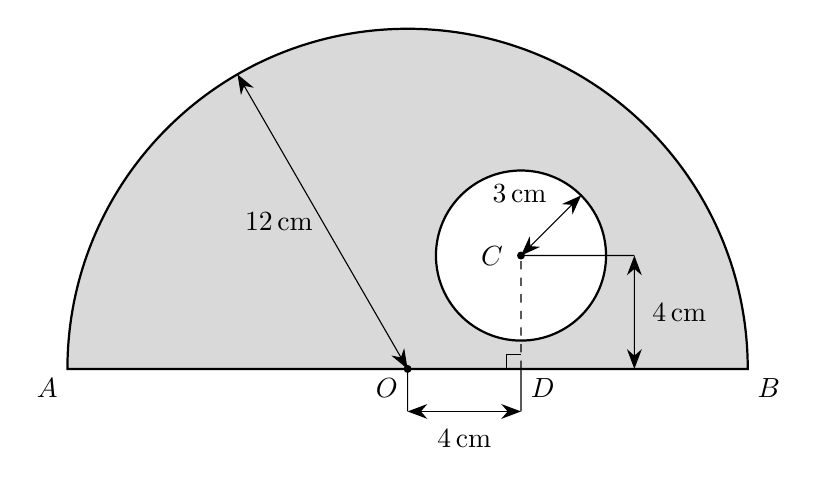
\begin{tikzpicture}[scale=0.36]
\def\rad{12}
\def\holeRad{3}
\def\offsetX{4}
\def\offsetY{4}
\def\markSize{0.5}
\def\dimDrop{1.5}
\def\dimShift{4}
\coordinate (O) at (0,0);
\coordinate (A) at (-\rad,0);
\coordinate (B) at (\rad,0);
\coordinate (D) at (\offsetX,0);
\coordinate (C) at ($(D)+(0,\offsetY)$);
\coordinate (P) at (120:\rad);
\coordinate (Q) at ($(C)+(45:\holeRad)$);
\coordinate (Od) at ($(O)+(0,-\dimDrop)$);
\coordinate (Dd) at ($(D)+(0,-\dimDrop)$);
\coordinate (Dv) at ($(D)+(\dimShift,0)$);
\coordinate (Cv) at ($(C)+(\dimShift,0)$);
\path[fill=gray!30,even odd rule] (A) arc[start angle=180,end angle=0,radius=\rad] -- cycle (C) circle (\holeRad);
\draw[thick,black] (A) arc[start angle=180,end angle=0,radius=\rad] -- cycle;
\draw[thick,black] (C) circle (\holeRad);
\draw[dashed,black] (D) -- (C);
\draw[thin,black] (O)--(Od) (D)--(Dd) (D)--(Dv) (C)--(Cv);
\draw[{Stealth[length=2.5mm]}-{Stealth[length=2.5mm]},black] (Od)--(Dd) node[midway,below=3pt] {$4\,\mathrm{cm}$};
\draw[{Stealth[length=2.5mm]}-{Stealth[length=2.5mm]},black] (Dv)--(Cv) node[midway,right=3pt] {$4\,\mathrm{cm}$};
\draw[black] ($(D)+(-\markSize,0)$) -- ($(D)+(-\markSize,\markSize)$) -- ($(D)+(0,\markSize)$);
\draw[{Stealth[length=2.5mm]}-{Stealth[length=2.5mm]},black] (O) -- (P) node[midway,left] {$12\,\mathrm{cm}$};
\draw[{Stealth[length=2.5mm]}-{Stealth[length=2.5mm]},black] (C) -- (Q) node[pos=0.65,above left=2pt] {$3\,\mathrm{cm}$};
\foreach \p in {O,C} {\fill[black] (\p) circle (4pt);}
\node[below left] at (A) {$A$};
\node[below right] at (B) {$B$};
\node[below left] at (O) {$O$};
\node[below right] at (D) {$D$};
\node[left=3pt] at (C) {$C$};
\end{tikzpicture}
\end{figure}


A uniform semicircular lamina has radius $12\,\mathrm{cm}$ and diameter $AB$, with midpoint $O$. \\
A circular hole of radius $3\,\mathrm{cm}$ is cut from the lamina. \\
Its centre $C$ is $4\,\mathrm{cm}$ above a point $D$ on $OB$, where $OD=4\,\mathrm{cm}$ and $CD$ is perpendicular to $AB$, as shown in the diagram above. \\

The remaining lamina is freely suspended from $B$ and hangs in equilibrium. \\

Determine the acute angle that $AB$ makes with the vertical, giving your answer to the nearest $0.1^\circ$. \\

You may use the result that the centre of mass of a uniform semicircular lamina of radius $r$ is on its axis of symmetry at a distance $\frac{4r}{3\pi}$ from its diameter. \marks{9} \\

\vspace*{10pt}

\begin{djsSolution}
Take \(O\) as the origin, with the \(x\)-axis along \(OB\) and the \(y\)-axis perpendicular to \(AB\), towards the semicircle. Measure coordinates in centimetres, so \(B=(12,0)\) and \(C=(4,4)\).

The centre of mass of a uniform semicircular lamina of radius \(r\) lies on its axis of symmetry, a distance \(\frac{4r}{3\pi}\) from its diameter. Thus the centre of mass of the complete semicircle has coordinates
\[
\left(0,\dfrac{4\times12}{3\pi}\right)=\left(0,\dfrac{16}{\pi}\right)
\]

Let \(\mathcal{A}_s\), \(\mathcal{A}_h\) and \(\mathcal{A}\) denote the areas of the complete semicircle, the hole and the remaining lamina respectively. Then
\begin{align*}
\mathcal{A}_s&=\dfrac12\pi(12)^2=72\pi\,\mathrm{cm^2}\\
\mathcal{A}_h&=\pi(3)^2=9\pi\,\mathrm{cm^2}\\
\mathcal{A}&=72\pi-9\pi=63\pi\,\mathrm{cm^2}
\end{align*}

Let the remaining lamina have centre of mass \(G\), with coordinates \((\bar{x},\bar{y})\). The lamina is uniform, so areas can be used as weights. If piece \(i\) has area \(\mathcal{A}_i\) and centre of mass \((x_i,y_i)\), then
\[
\mathcal{A}\bar{x}=\sum\mathcal{A}_ix_i,\qquad \mathcal{A}\bar{y}=\sum\mathcal{A}_iy_i
\]

where \(\mathcal{A}=\sum\mathcal{A}_i\), with the area of a removed piece counted as negative.

Taking moments about the \(y\)-axis:
\begin{align*}
63\pi\bar{x}&=72\pi\times0-9\pi\times4\\
&=-36\pi\\
\bar{x}&=-\dfrac47\,\mathrm{cm}
\end{align*}

Taking moments about the \(x\)-axis:
\begin{align*}
63\pi\bar{y}&=72\pi\times\dfrac{16}{\pi}-9\pi\times4\\
&=1152-36\pi\\
\bar{y}&=\dfrac{128-4\pi}{7\pi}\,\mathrm{cm}
\end{align*}

When suspended in equilibrium, \(G\) lies vertically below \(B\). Hence the required acute angle \(\theta\) is the angle between \(BA\) and \(BG\). Using the perpendicular distances from \(B\) to \(G\):
\begin{align*}
\tan\theta&=\dfrac{\bar{y}}{12-\bar{x}}\\
&=\dfrac{\dfrac{128-4\pi}{7\pi}}{12+\dfrac47}\\
&=\dfrac{32-\pi}{22\pi}\\
\theta&=\arctan\left(\dfrac{32-\pi}{22\pi}\right)\approx22.7^\circ\qquad\text{(1 d.p.)}
\end{align*}

\end{djsSolution}

\newpage

% ---- Question 2 ----
\questionitem
% [Source: _QBT___Solns__Centre_of_Mass_of_Circular_Laminae, Q2]

\begin{figure}[H]
    \centering
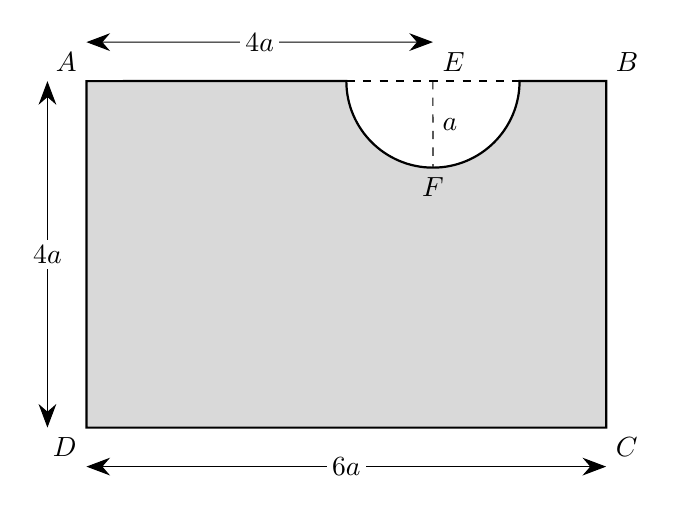
\begin{tikzpicture}[scale=1.1]
\def\a{1}
\def\dimoff{0.45}
\coordinate (D) at (0,0);
\coordinate (A) at ($(D)+(0,4*\a)$);
\coordinate (B) at ($(A)+(6*\a,0)$);
\coordinate (C) at ($(D)+(6*\a,0)$);
\coordinate (E) at ($(A)+(4*\a,0)$);
\coordinate (F) at ($(E)+(0,-\a)$);
\coordinate (L) at ($(E)+(-\a,0)$);
\coordinate (R) at ($(E)+(\a,0)$);
\fill[gray!30] (A) -- (L) arc[start angle=180,end angle=360,radius=\a] -- (B) -- (C) -- (D) -- cycle;
\draw[thick,black] (A) -- (L) arc[start angle=180,end angle=360,radius=\a] -- (B) -- (C) -- (D) -- cycle;
\draw[dashed,black] (L) -- (R);
\draw[dashed,black] (E) -- (F) node[midway,right] {$a$};
\draw[{Stealth[length=3mm]}-{Stealth[length=3mm]}] ($(D)+(0,-\dimoff)$) -- ($(C)+(0,-\dimoff)$) node[midway,fill=white,inner sep=2pt] {$6a$};
\draw[{Stealth[length=3mm]}-{Stealth[length=3mm]}] ($(D)+(-\dimoff,0)$) -- ($(A)+(-\dimoff,0)$) node[midway,fill=white,inner sep=2pt] {$4a$};
\draw[{Stealth[length=3mm]}-{Stealth[length=3mm]}] ($(A)+(0,\dimoff)$) -- ($(E)+(0,\dimoff)$) node[midway,fill=white,inner sep=2pt] {$4a$};
\node[above left] at (A) {$A$};
\node[above right] at (B) {$B$};
\node[below right] at (C) {$C$};
\node[below left] at (D) {$D$};
\node[above right] at (E) {$E$};
\node[below] at (F) {$F$};
\end{tikzpicture}
\end{figure}


A uniform rectangular lamina $ABCD$ has $AB=6a$ and $AD=4a$, where $a>0$. \\
A semicircular notch of radius $a$ is cut from the edge $AB$. \\
The centre $E$ of the semicircle lies on $AB$, with $AE=4a$, and the semicircle lies inside the rectangle, as shown in the diagram above. \\

You may use the result that the centre of mass of a uniform semicircular lamina of radius $r$ is a distance $\frac{4r}{3\pi}$ from its diameter. \\
\begin{enumerate}[label=\textbf{(\alph*)}]
\item
\begin{enumerate}[label=(\roman*)]
\item Show that the perpendicular distance of the centre of mass of the remaining lamina from $AD$ is
\[
\dfrac{4(36-\pi)}{48-\pi}a
\]
\item The remaining lamina is freely suspended from $A$ and hangs in equilibrium. Calculate the acute angle that $AB$ makes with the downward vertical, giving your answer to the nearest $0.1^\circ$.
\end{enumerate}
\end{enumerate}
\marks[-10pt]{9}

\vspace*{10pt}

\begin{djsSolution}
\begin{enumerate}[label=\textbf{(\alph*)}, start=1]
\item
\begin{enumerate}[label=(\roman*), start=1]
\item Take \(D\) as the origin, with the \(x\)-axis along \(DC\) and the \(y\)-axis along \(DA\). Let the centre of mass of the remaining lamina be \(G(\bar{x},\bar{y})\).

The area \(\mathcal{A}\) of the remaining lamina is
\[
\mathcal{A}=(6a)(4a)-\dfrac12\pi a^2=\dfrac{48-\pi}{2}a^2
\]

The rectangle has its centre of mass at \(x=3a\). By symmetry, the removed semicircle has its centre of mass on the line through \(E\) perpendicular to \(AB\), so its \(x\)-coordinate is \(4a\).

The lamina is uniform, so areas can be used as weights. If piece \(i\) has area \(\mathcal{A}_i\) and centre of mass \((x_i,y_i)\), then
\[
\mathcal{A}\bar{x}=\sum\mathcal{A}_ix_i,\qquad \mathcal{A}\bar{y}=\sum\mathcal{A}_iy_i
\]

where \(\mathcal{A}=\sum\mathcal{A}_i\), with the area of a removed piece counted as negative.

Taking moments about \(AD\):
\begin{align*}
\mathcal{A}\bar{x}&=24a^2(3a)-\dfrac{\pi a^2}{2}(4a)\\
\dfrac{48-\pi}{2}a^2\bar{x}&=(72-2\pi)a^3\\
\bar{x}&=\dfrac{4(36-\pi)}{48-\pi}a
\end{align*}

\item The centre of mass of a uniform semicircular lamina of radius \(r\) lies on its axis of symmetry, a distance \(\frac{4r}{3\pi}\) from its diameter.

Thus the removed semicircle has its centre of mass at height \(4a-\frac{4a}{3\pi}\) above \(DC\). The original rectangle has its centre of mass at height \(2a\). Taking moments about \(DC\):
\begin{align*}
\mathcal{A}\bar{y}&=24a^2(2a)-\dfrac{\pi a^2}{2}\left(4a-\dfrac{4a}{3\pi}\right)\\
\dfrac{48-\pi}{2}a^2\bar{y}&=48a^3-2\pi a^3+\dfrac23a^3\\
\bar{y}&=\dfrac{292-12\pi}{3(48-\pi)}a
\end{align*}

Let \(h\) be the perpendicular distance of \(G\) below \(AB\). Then
\begin{align*}
h&=4a-\bar{y}\\
&=\dfrac{12(48-\pi)-(292-12\pi)}{3(48-\pi)}a\\
&=\dfrac{284}{3(48-\pi)}a
\end{align*}

When the lamina hangs in equilibrium, \(G\) is vertically below \(A\), so \(AG\) gives the downward vertical. Let \(\theta\) be the acute angle between \(AB\) and \(AG\). Using the right-angled triangle with components \(\bar{x}\) parallel to \(AB\) and \(h\) perpendicular to \(AB\), together with part (a)(i):
\begin{align*}
\tan\theta&=\dfrac{h}{\bar{x}}\\
&=\dfrac{284}{3(48-\pi)}\times\dfrac{48-\pi}{4(36-\pi)}\\
&=\dfrac{71}{3(36-\pi)}\\
\theta&=\arctan\left(\dfrac{71}{3(36-\pi)}\right)\approx35.8^\circ\qquad\text{(1 d.p.)}
\end{align*}

\end{enumerate}
\end{enumerate}
\end{djsSolution}

\newpage

% ---- Question 3 ----
\questionitem
% [Source: _QBT___Solns__Centre_of_Mass_of_Circular_Laminae, Q3]

\begin{figure}[H]
    \centering
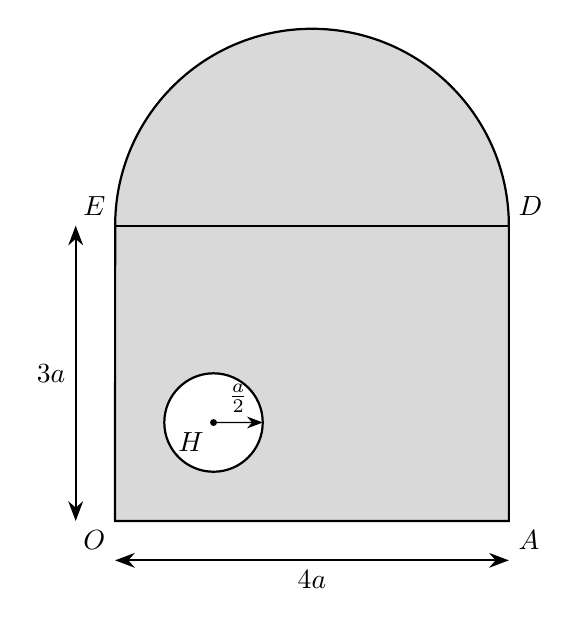
\begin{tikzpicture}[scale=1.25]
\def\a{1}
\def\width{4*\a}
\def\height{3*\a}
\def\semirad{2*\a}
\def\holerad{0.5*\a}
\def\dimoff{0.4*\a}
\coordinate (O) at (0,0);
\coordinate (A) at (\width,0);
\coordinate (D) at (\width,\height);
\coordinate (E) at (0,\height);
\coordinate (H) at (\a,\a);
\coordinate (R) at ($(H)+(0:\holerad)$);
\path[fill=gray!30,even odd rule] (O) -- (A) -- (D) arc[start angle=0,end angle=180,radius=\semirad] -- cycle (H) circle (\holerad);
\draw[thick,black] (O) -- (A) -- (D) arc[start angle=0,end angle=180,radius=\semirad] -- cycle;
\draw[thick,black] (E) -- (D);
\draw[thick,black] (H) circle (\holerad);
\draw[-{Stealth[length=2mm]},black] (H) -- (R) node[midway,above] {$\frac{a}{2}$};
\fill[black] (H) circle (1pt);
\node[below left] at (H) {$H$};
\node[below left] at (O) {$O$};
\node[below right] at (A) {$A$};
\node[above right] at (D) {$D$};
\node[above left] at (E) {$E$};
\draw[{Stealth[length=2.5mm]}-{Stealth[length=2.5mm]},thick] ($(O)+(0,-\dimoff)$) -- node[midway,below] {$4a$} ($(A)+(0,-\dimoff)$);
\draw[{Stealth[length=2.5mm]}-{Stealth[length=2.5mm]},thick] ($(O)+(-\dimoff,0)$) -- node[midway,left] {$3a$} ($(E)+(-\dimoff,0)$);
\end{tikzpicture}
\end{figure}


A uniform lamina is made by joining a rectangle $OADE$ to a semicircle along its diameter $ED$, and then removing a circular disc from the rectangular portion, as shown in the diagram above. \\

The rectangle has $OA=4a$ and $OE=3a$, where $a>0$. \\
The removed disc has radius $\frac{a}{2}$ and centre $H$, which is a distance $a$ from each of the sides $OE$ and $OA$. \\

You may use the result that the centre of mass of a uniform semicircular lamina of radius $r$ is a distance $\frac{4r}{3\pi}$ from its diameter. \\
\begin{enumerate}[label=\textbf{(\alph*)}]
\item Find, in terms of $a$ and $\pi$, the distance of the centre of mass of the remaining lamina from
\begin{enumerate}[label=(\roman*)]
\item $OE$,
\item $OA$.
\end{enumerate}
\marks[-10pt]{6}
\end{enumerate}
The remaining lamina is freely suspended from $A$ and hangs in equilibrium. \\
The angle between $AO$ and the downward vertical is $\alpha$. \\
\begin{enumerate}[label=\textbf{(\alph*)}, resume]
\item Find the exact value of $\tan\alpha$. \marks{2} \\
\end{enumerate}

\vspace*{10pt}

\begin{djsSolution}
\begin{enumerate}[label=\textbf{(\alph*)}, start=1]
\item
\begin{enumerate}[label=(\roman*), start=1]
\item Let the centre of mass be \(G\), at distances \(\bar{x}\) from \(OE\) and \(\bar{y}\) from \(OA\). The lamina is uniform, so areas can be used as weights. If piece \(i\) has area \(\mathcal{A}_i\) and its centre of mass is at distances \(x_i\) from \(OE\) and \(y_i\) from \(OA\), then
\[
\mathcal{A}\bar{x}=\sum\mathcal{A}_ix_i,\qquad \mathcal{A}\bar{y}=\sum\mathcal{A}_iy_i
\]

where \(\mathcal{A}=\sum\mathcal{A}_i\), with the area of a removed piece counted as negative.

The semicircle has radius \(2a\), so the remaining area \(\mathcal{A}\) is
\begin{align*}
\mathcal{A}&=(4a)(3a)+\dfrac12\pi(2a)^2-\pi\left(\dfrac a2\right)^2\\
&=\dfrac{a^2(48+7\pi)}4
\end{align*}

The rectangle and semicircle each have their centre of mass at distance \(2a\) from \(OE\); the removed disc has its centre at distance \(a\). Taking moments about \(OE\):
\begin{align*}
\mathcal{A}\bar{x}&=12a^2(2a)+2\pi a^2(2a)-\dfrac{\pi a^2}{4}(a)\\
&=\dfrac{a^3(96+15\pi)}4\\
\bar{x}&=\dfrac{a(96+15\pi)}{48+7\pi}
\end{align*}

\item The centre of mass of a uniform semicircular lamina of radius \(r\) lies on its axis of symmetry, a distance \(\frac{4r}{3\pi}\) from its diameter. Here the diameter is \(3a\) above \(OA\), so the semicircle's centre of mass is at distance
\[
3a+\dfrac{4(2a)}{3\pi}=3a+\dfrac{8a}{3\pi}
\]

from \(OA\). The rectangle's centre is at distance \(\frac{3a}{2}\), and the removed disc's centre is at distance \(a\). Taking moments about \(OA\):
\begin{align*}
\mathcal{A}\bar{y}&=12a^2\left(\dfrac{3a}{2}\right)+2\pi a^2\left(3a+\dfrac{8a}{3\pi}\right)-\dfrac{\pi a^2}{4}(a)\\
&=a^3\left(18+6\pi+\dfrac{16}{3}-\dfrac{\pi}{4}\right)\\
&=\dfrac{a^3(280+69\pi)}{12}\\
\bar{y}&=\dfrac{a(280+69\pi)}{3(48+7\pi)}
\end{align*}

\end{enumerate}
\item In equilibrium, \(G\) lies vertically below \(A\), so \(\alpha\) is the angle between \(AO\) and \(AG\). Relative to the original diagram, the distances from \(A\) to \(G\) parallel and perpendicular to \(AO\) are \(4a-\bar{x}\) and \(\bar{y}\), respectively. Then
\begin{align*}
4a-\bar{x}&=4a-\dfrac{a(96+15\pi)}{48+7\pi}\\
&=\dfrac{a(96+13\pi)}{48+7\pi}\\
\tan\alpha&=\dfrac{\bar{y}}{4a-\bar{x}}\\
&=\dfrac{280+69\pi}{3(96+13\pi)}
\end{align*}

\end{enumerate}
\end{djsSolution}

\newpage

% ---- Question 4 ----
\questionitem
% [Source: _QBT___Solns__Centre_of_Mass_of_Circular_Laminae, Q4]

\begin{figure}[H]
    \centering
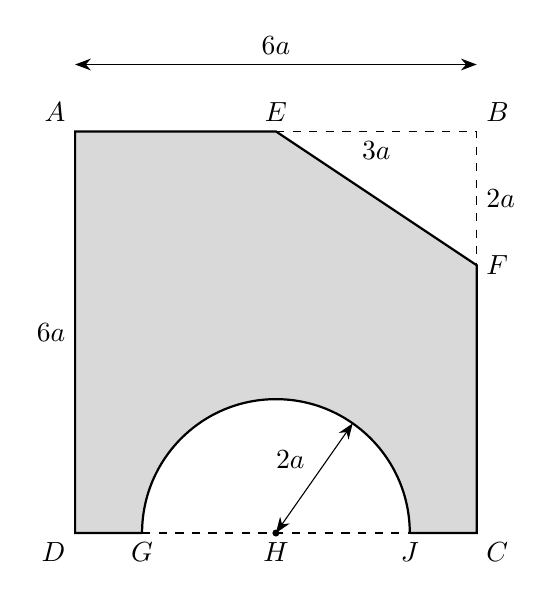
\begin{tikzpicture}[scale=0.85]
\def\s{6}
\def\leg{3}
\def\drop{2}
\def\rad{2}
\def\dimoff{1}
\def\radiusang{55}
\coordinate (D) at (0,0);
\coordinate (A) at (0,\s);
\coordinate (B) at (\s,\s);
\coordinate (C) at (\s,0);
\coordinate (E) at ({\s-\leg},\s);
\coordinate (F) at (\s,{\s-\drop});
\coordinate (H) at ({\s/2},0);
\coordinate (G) at ($(H)+(-\rad,0)$);
\coordinate (J) at ($(H)+(\rad,0)$);
\coordinate (R) at ($(H)+(\radiusang:\rad)$);
\fill[gray!30] (A)--(E)--(F)--(C)--(D)--cycle;
\fill[white] (G) arc[start angle=180,end angle=0,radius=\rad] -- cycle;
\draw[thick,black] (G)--(D)--(A)--(E)--(F)--(C)--(J);
\draw[thick,black] (G) arc[start angle=180,end angle=0,radius=\rad];
\draw[dashed,black] (E)--(B)--(F);
\draw[dashed,black] (G)--(J);
\draw[{Stealth[length=2mm]}-{Stealth[length=2mm]}] ($(A)+(0,\dimoff)$)--($(B)+(0,\dimoff)$) node[midway,above] {$6a$};
\path (A)--(D) node[midway,left] {$6a$};
\path (E)--(B) node[midway,below] {$3a$};
\path (B)--(F) node[midway,right] {$2a$};
\draw[{Stealth[length=2mm]}-{Stealth[length=2mm]}] (H)--(R) node[midway,above left] {$2a$};
\fill[black] (H) circle (1.5pt);
\foreach \p/\pos in {A/above left,B/above right,C/below right,D/below left,E/above,F/right,G/below,H/below,J/below} {
  \node[\pos] at (\p) {$\p$};
}
\end{tikzpicture}
\end{figure}


A uniform square lamina $ABCD$ has side $6a$. \\
A template $T$, shown shaded in the diagram above, is made by removing two portions of the lamina. \\

The first portion is the right-angled triangle $EBF$, where $E$ lies on $AB$, $F$ lies on $BC$, $EB=3a$ and $BF=2a$. \\

The second portion is a semicircle of radius $2a$. \\
Its centre $H$ is the midpoint of $DC$, its diameter lies on $DC$, and the semicircle lies inside the square. \\

\begin{enumerate}[label=\textbf{(\alph*)}]
\item Find the distances of the centre of mass of $T$ from $AD$ and from $DC$, giving both answers exactly in terms of $a$ and $\pi$. \marks{6} \\
\end{enumerate}
The template is now freely suspended from $A$ and hangs in equilibrium in a vertical plane. \\
\begin{enumerate}[label=\textbf{(\alph*)}, resume]
\item Find the acute angle between $AD$ and the vertical, giving your answer to the nearest $0.1^\circ$. \marks{3} \\
\end{enumerate}

\vspace*{10pt}

\begin{djsSolution}
\begin{enumerate}[label=\textbf{(\alph*)}, start=1]
\item
Take \(D\) as the origin, with the positive \(x\)-axis along \(DC\) and the positive \(y\)-axis along \(DA\). Then \(\bar{x}\) and \(\bar{y}\) are the required distances from \(AD\) and \(DC\), respectively.

The centre of mass of a uniform triangular lamina is \(\frac23\) of the way along a median from the vertex, so its coordinates are the means of the vertices' coordinates. Here \(E(3a,6a)\), \(B(6a,6a)\) and \(F(6a,4a)\), so the triangle's centre of mass is
\[
\left(\dfrac{3a+6a+6a}{3},\dfrac{6a+6a+4a}{3}\right)
=\left(5a,\dfrac{16a}{3}\right)
\]

The centre of mass of a uniform semicircular lamina of radius \(r\) lies on its axis of symmetry, a distance \(\frac{4r}{3\pi}\) from its diameter. Thus the areas and centre-of-mass coordinates are
\[
\renewcommand{\arraystretch}{1.5}
\setlength{\arraycolsep}{8pt}
\begin{array}{c|c|c|c}
\text{Portion} & \text{Area} & x & y\\ \hline
\text{Square} & 36a^2 & 3a & 3a\\
\text{Triangle removed} & -3a^2 & 5a & \tfrac{16a}{3}\\
\text{Semicircle removed} & -2\pi a^2 & 3a & \tfrac{8a}{3\pi}
\end{array}
\]

The lamina is uniform, so areas can be used as weights. If piece \(i\) has area \(\mathcal{A}_i\) and centre of mass \((x_i,y_i)\), then
\[
\mathcal{A}\bar{x}=\sum\mathcal{A}_ix_i,\qquad \mathcal{A}\bar{y}=\sum\mathcal{A}_iy_i
\]

where \(\mathcal{A}=\sum\mathcal{A}_i\), with the area of a removed piece counted as negative.

The remaining area is
\[
\mathcal{A}=36a^2-3a^2-2\pi a^2=(33-2\pi)a^2
\]

Taking moments about \(AD\) and about \(DC\):
\begin{align*}
(33-2\pi)a^2\bar{x}
&=36a^2(3a)-3a^2(5a)-2\pi a^2(3a)\\
&=(93-6\pi)a^3\\
\bar{x}&=\dfrac{(93-6\pi)a}{33-2\pi}\\
(33-2\pi)a^2\bar{y}
&=36a^2(3a)-3a^2\left(\dfrac{16a}{3}\right)
-2\pi a^2\left(\dfrac{8a}{3\pi}\right)\\
&=\left(108-16-\dfrac{16}{3}\right)a^3
=\dfrac{260a^3}{3}\\
\bar{y}&=\dfrac{260a}{3(33-2\pi)}
\end{align*}

\item When the template hangs in equilibrium, its centre of mass is vertically below \(A\). Let \(\theta\) be the acute angle between \(AD\) and the vertical.

The centre of mass is \(\bar{x}\) perpendicular to \(AD\), and \(6a-\bar{y}\) along \(AD\) from \(A\). Using part (a):
\begin{align*}
\tan\theta
&=\dfrac{\bar{x}}{6a-\bar{y}}\\
&=\dfrac{93-6\pi}{6(33-2\pi)-\dfrac{260}{3}}\\
&=\dfrac{279-18\pi}{334-36\pi}\\
\theta&=\arctan\left(\dfrac{279-18\pi}{334-36\pi}\right)
\approx45.2^\circ\qquad\text{(1 d.p.)}
\end{align*}

\end{enumerate}
\end{djsSolution}

\newpage

% ---- Question 5 ----
\questionitem
% [Source: _QBT___Solns__Centre_of_Mass_of_Circular_Laminae, Q5]

\begin{figure}[H]
    \centering
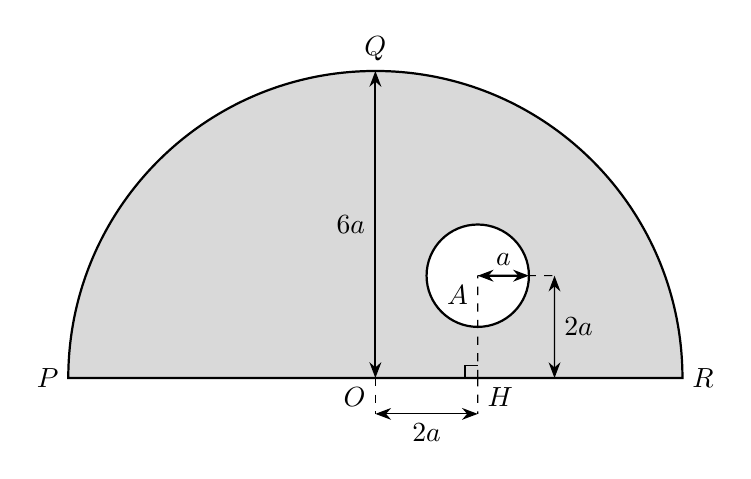
\begin{tikzpicture}[scale=0.65]
\def\a{1}
\def\rad{6*\a}
\def\holerad{\a}
\def\offset{2*\a}
\def\dimdrop{0.7*\a}
\def\dimshift{1.5*\a}
\def\marksize{0.25*\a}
\coordinate (O) at (0,0);
\coordinate (P) at (180:\rad);
\coordinate (Q) at (90:\rad);
\coordinate (R) at (0:\rad);
\coordinate (H) at (\offset,0);
\coordinate (A) at ($(H)+(0,\offset)$);
\coordinate (Ar) at ($(A)+(\holerad,0)$);
\coordinate (Od) at ($(O)+(0,-\dimdrop)$);
\coordinate (Hd) at ($(H)+(0,-\dimdrop)$);
\coordinate (Hv) at ($(H)+(\dimshift,0)$);
\coordinate (Av) at ($(A)+(\dimshift,0)$);
\fill[gray!30] (P) arc[start angle=180,end angle=0,radius=\rad] -- cycle;
\fill[white] (A) circle (\holerad);
\draw[thick,black] (P) arc[start angle=180,end angle=0,radius=\rad] -- cycle;
\draw[thick,black] (A) circle (\holerad);
\draw[dashed,black] (H) -- (A);
\draw[{Stealth[length=2mm]}-{Stealth[length=2mm]},thick,black] (O) -- (Q) node[midway,left] {$6a$};
\draw[{Stealth[length=2mm]}-{Stealth[length=2mm]},thick,black] (A) -- (Ar) node[midway,above] {$a$};
\foreach \point/\end in {O/Od,H/Hd,H/Hv,A/Av} {
  \draw[dashed,black] (\point) -- (\end);
}
\draw[{Stealth[length=2mm]}-{Stealth[length=2mm]},black] (Od) -- (Hd) node[midway,below] {$2a$};
\draw[{Stealth[length=2mm]}-{Stealth[length=2mm]},black] (Hv) -- (Av) node[midway,right] {$2a$};
\draw[black] ($(H)+(-\marksize,0)$) -- ($(H)+(-\marksize,\marksize)$) -- ($(H)+(0,\marksize)$);
\node[left] at (P) {$P$};
\node[above] at (Q) {$Q$};
\node[right] at (R) {$R$};
\node[below left] at (O) {$O$};
\node[below right] at (H) {$H$};
\node[below left] at (A) {$A$};
\end{tikzpicture}
\end{figure}


A uniform semicircular lamina has centre $O$, radius $6a$ and diameter $PR$. \\
A circular disc of radius $a$ is removed to form the lamina $L$ shown shaded in the diagram above. \\
The centre of the removed disc is $A$. \\
The point $H$ lies on $OR$, with $OH=2a$, $HA=2a$ and $HA$ perpendicular to $PR$. \\

Take $O$ as the origin, with the positive $x$-axis directed towards $R$ and the positive $y$-axis directed towards $Q$. \\
\begin{enumerate}[label=\textbf{(\alph*)}]
\item Find the exact coordinates of the centre of mass of $L$. \marks{6} \\
\end{enumerate}
The mass of $L$ is $M$. \\
A particle of mass $kM$ is attached at $P$. \\
The system is freely suspended from $R$ and hangs in equilibrium, with $P$ below $R$ and the diameter $PR$ making an acute angle of $\arctan\left(\frac{1}{6}\right)$ with the downward vertical through $R$. \\
\begin{enumerate}[label=\textbf{(\alph*)}, resume]
\item Find the exact value of $k$ and the magnitude of the supporting force at $R$ in terms of $M$ and $g$. \marks{6} \\
\end{enumerate}

\vspace*{10pt}

\begin{djsSolution}
\begin{enumerate}[label=\textbf{(\alph*)}, start=1]
\item The centre of mass of a uniform semicircular lamina of radius \(r\) lies on its axis of symmetry, a distance \(\frac{4r}{3\pi}\) from its diameter.

Thus the original semicircle has area and centre of mass
\[
\dfrac12\pi(6a)^2=18\pi a^2,
\qquad
\left(0,\dfrac{4(6a)}{3\pi}\right)=\left(0,\dfrac{8a}{\pi}\right)
\]

The removed disc has area \(\pi a^2\) and centre of mass \(A(2a,2a)\). Therefore the area of \(L\) is
\[
18\pi a^2-\pi a^2=17\pi a^2
\]

Let the centre of mass of \(L\) be \((\bar{x},\bar{y})\). The lamina is uniform, so areas can be used as weights. If piece \(i\) has area \(\mathcal{A}_i\) and centre of mass \((x_i,y_i)\), then
\[
\mathcal{A}\bar{x}=\sum\mathcal{A}_ix_i,\qquad \mathcal{A}\bar{y}=\sum\mathcal{A}_iy_i
\]

where \(\mathcal{A}=\sum\mathcal{A}_i\), with the area of a removed piece counted as negative.

Taking moments about the \(y\)-axis and about the \(x\)-axis:
\begin{align*}
17\pi a^2\bar{x}
&=18\pi a^2(0)-\pi a^2(2a)
=-2\pi a^3\\
17\pi a^2\bar{y}
&=18\pi a^2\left(\dfrac{8a}{\pi}\right)-\pi a^2(2a)
=(144-2\pi)a^3
\end{align*}

Dividing by \(17\pi a^2\), the exact coordinates are
\[
\left(-\dfrac{2a}{17},\dfrac{(144-2\pi)a}{17\pi}\right)
\]

\item Write \(\theta=\arctan\left(\frac16\right)\), so \(\tan\theta=\frac16\).

Relative to \(R\), the centre of mass of \(L\) is a distance \(6a-\bar{x}\) towards \(P\) and a distance \(\bar{y}\) perpendicular to \(PR\), on the \(Q\) side. Also, \(RP=12a\).

Resolve the weights parallel and perpendicular to \(PR\). The parallel component of the lamina's weight has magnitude \(Mg\cos\theta\), while the perpendicular components have magnitudes \(Mg\sin\theta\) and \(kMg\sin\theta\). Taking moments about \(R\):
\[
Mg\bar{y}\cos\theta
=Mg(6a-\bar{x})\sin\theta+kMg(12a)\sin\theta
\]

Dividing by \(Mg\sin\theta\) gives
\[
\bar{y}\cot\theta=6a-\bar{x}+12ak
\]

Substituting the coordinates from part (a) and \(\cot\theta=6\):
\begin{align*}
6\left(\dfrac{(144-2\pi)a}{17\pi}\right)
&=6a+\dfrac{2a}{17}+12ak\\
\dfrac{(864-12\pi)a}{17\pi}
&=\dfrac{104a}{17}+12ak\\
864-12\pi&=104\pi+204\pi k\\
204\pi k&=864-116\pi\\
k&=\dfrac{216-29\pi}{51\pi}
\end{align*}

The supporting force \(F\) balances the total weight of the system, so
\begin{align*}
F&=(M+kM)g\\
&=\left(1+\dfrac{216-29\pi}{51\pi}\right)Mg\\
&=\dfrac{216+22\pi}{51\pi}Mg
\end{align*}

\end{enumerate}
\end{djsSolution}

\newpage

% ---- Question 6 ----
\questionitem
% [Source: _QBT___Solns__Centre_of_Mass_of_Circular_Laminae, Q6]

\begin{figure}[H]
    \centering
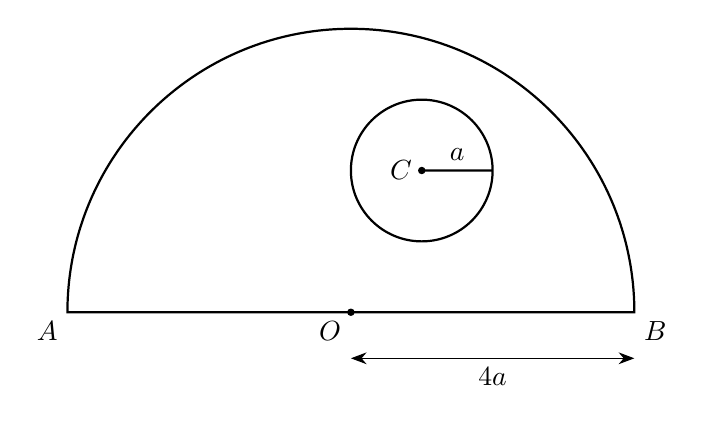
\begin{tikzpicture}[scale=0.9]
\def\rad{4}
\def\hole{1}
\def\cx{1}
\def\cy{2}
\def\dimdrop{0.65}
\coordinate (O) at (0,0);
\coordinate (A) at (-\rad,0);
\coordinate (B) at (\rad,0);
\coordinate (C) at (\cx,\cy);
\coordinate (E) at ($(C)+(\hole,0)$);
\draw[thick,black] (B) arc[start angle=0,end angle=180,radius=\rad] -- cycle;
\draw[thick,black] (C) circle (\hole);
\draw[thick,black] (C)--(E) node[midway,above] {$a$};
\foreach \p in {O,C} {\fill[black] (\p) circle (1.5pt);}
\node[below left] at (A) {$A$};
\node[below right] at (B) {$B$};
\node[below left] at (O) {$O$};
\node[left] at (C) {$C$};
\coordinate (Om) at ($(O)+(0,-\dimdrop)$);
\coordinate (Bm) at ($(B)+(0,-\dimdrop)$);
\draw[{Stealth[length=2mm]}-{Stealth[length=2mm]}] (Om)--(Bm) node[midway,below] {$4a$};
\end{tikzpicture}
\end{figure}


A uniform semicircular lamina has radius $4a$ and diameter $AB$, whose midpoint is $O$. \\
A circular hole of radius $a$ is cut from the lamina. \\
In the orientation shown above, take $O$ as the origin, the positive $x$-direction along $OB$ and the positive $y$-direction perpendicular to $AB$ towards the semicircular arc. \\
The centre $C$ of the hole has coordinates $(a,2a)$. \\
\begin{enumerate}[label=\textbf{(\alph*)}]
\item Show that the centre of mass $G$ of the remaining lamina has coordinates
\[
\left(-\dfrac{a}{7},\ \dfrac{(128-6\pi)a}{21\pi}\right)
\] \marks[-30pt]{6}
\end{enumerate}
The remaining lamina has mass $7\,\mathrm{kg}$. \\
It is freely pivoted at $A$ and turned so that $AB$ is vertical, with $A$ above $B$ and the semicircular arc to the right of $AB$, as shown in the diagram below. \\
A light string attached to $B$ holds the lamina in equilibrium. \\
The string lies in the plane of the lamina and makes an angle of $30^\circ$ below the horizontal. \\
\begin{figure}[H]
    \centering
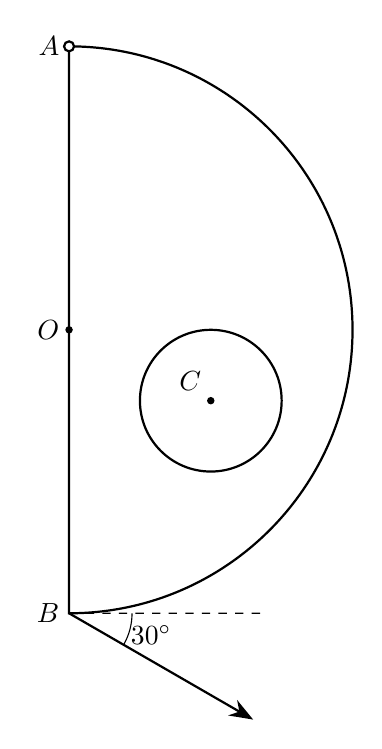
\begin{tikzpicture}[scale=0.9]
\def\rad{4}
\def\hole{1}
\def\cx{1}
\def\cy{2}
\def\stringlen{3}
\def\horizlen{2.8}
\def\ang{30}
\coordinate (O) at (0,0);
\coordinate (A) at (0,\rad);
\coordinate (B) at (0,-\rad);
\coordinate (C) at (\cy,-\cx);
\coordinate (H) at ($(B)+(\horizlen,0)$);
\coordinate (S) at ($(B)+(-\ang:\stringlen)$);
\draw[thick,black] (B) arc[start angle=-90,end angle=90,radius=\rad] -- cycle;
\draw[thick,black] (C) circle (\hole);
\draw[dashed,black] (B)--(H);
\draw[-{Stealth[length=3mm]},thick,black] (B)--(S);
\pic["$30^\circ$",draw,angle radius=8mm,angle eccentricity=1.35] {angle=S--B--H};
\foreach \p in {O,C} {\fill[black] (\p) circle (1.5pt);}
\draw[thick,fill=white] (A) circle (2pt);
\foreach \p in {A,B,O} {\node[left] at (\p) {$\p$};}
\node[above left] at (C) {$C$};
\end{tikzpicture}
\end{figure}


\begin{enumerate}[label=\textbf{(\alph*)}, resume]
\item Calculate the tension in the string. \marks{3} \\
\item Find the magnitude of the force exerted on the lamina by the pivot at $A$ and the angle this force makes with the upward vertical, stating on which side of the vertical it acts. \marks{5} \\
\end{enumerate}

\vspace*{10pt}

\begin{djsSolution}
\begin{enumerate}[label=\textbf{(\alph*)}, start=1]
\item
The centre of mass of a uniform semicircular lamina of radius \(r\) lies on its axis of symmetry, a distance \(\frac{4r}{3\pi}\) from its diameter. Thus the original lamina has centre of mass
\[
\left(0,\dfrac{4(4a)}{3\pi}\right)=\left(0,\dfrac{16a}{3\pi}\right)
\]

The areas of the original semicircle and the removed disc are
\[
\dfrac12\pi(4a)^2=8\pi a^2,
\qquad \pi a^2
\]

so the remaining lamina has area \(7\pi a^2\).

Let the centre of mass of the remaining lamina be \(G(\bar{x},\bar{y})\). The lamina is uniform, so areas can be used as weights. If piece \(i\) has area \(\mathcal{A}_i\) and centre of mass \((x_i,y_i)\), then
\[
\mathcal{A}\bar{x}=\sum\mathcal{A}_ix_i,\qquad \mathcal{A}\bar{y}=\sum\mathcal{A}_iy_i
\]

where \(\mathcal{A}=\sum\mathcal{A}_i\), with the area of a removed piece counted as negative.

Taking moments about the \(y\)-axis gives
\begin{align*}
7\pi a^2\bar{x}&=8\pi a^2(0)-\pi a^2(a)\\
7\bar{x}&=-a\\
\bar{x}&=-\dfrac{a}{7}
\end{align*}

Similarly, taking moments about the \(x\)-axis gives
\begin{align*}
7\pi a^2\bar{y}&=8\pi a^2\left(\dfrac{16a}{3\pi}\right)-\pi a^2(2a)\\
7\bar{y}&=\dfrac{128a}{3\pi}-2a\\
\bar{y}&=\dfrac{(128-6\pi)a}{21\pi}
\end{align*}

Hence \(G\) has coordinates
\[
\left(-\dfrac{a}{7},\ \dfrac{(128-6\pi)a}{21\pi}\right)
\]

\end{enumerate}
\begin{enumerate}[label=\textbf{(\alph*)}, start=2]
\item
The lamina has been turned through \(90^\circ\) clockwise, so the original \(y\)-coordinate of \(G\) is now its horizontal distance to the right of \(AB\).

The tension \(T\) has horizontal component \(T\cos30^\circ\), acting at \(B\), where \(AB=8a\). Its vertical component acts along \(AB\), so has no moment about \(A\).

Taking moments about \(A\), and using part (a):
\begin{align*}
8aT\cos30^\circ&=7g\left(\dfrac{(128-6\pi)a}{21\pi}\right)\\
T&=\dfrac{7g}{8\cos30^\circ}\times\dfrac{128-6\pi}{21\pi}
\end{align*}

Using \(g=9.8\,\mathrm{m\,s^{-2}}\), the tension is
\[
T\approx16.4\,\mathrm{N}
\]

\item Let the pivot force have components \(R_x\) horizontally to the right and \(R_y\) vertically upwards. Resolving horizontally and vertically for equilibrium:
\begin{align*}
R_x+T\cos30^\circ&=0\\
R_y-T\sin30^\circ-7g&=0
\end{align*}

Thus the pivot force acts to the left and upwards, with components
\[
R_x=-T\cos30^\circ,
\qquad R_y=7g+T\sin30^\circ
\]

Using the unrounded value of \(T\), its magnitude is
\begin{align*}
R&=\sqrt{(T\cos30^\circ)^2+(7g+T\sin30^\circ)^2}\\
&\approx78.1\,\mathrm{N}
\end{align*}

Let \(\theta\) be the angle the force makes with the upward vertical. Then
\begin{align*}
\tan\theta&=\dfrac{|R_x|}{R_y}
=\dfrac{T\cos30^\circ}{7g+T\sin30^\circ}\\
\theta&\approx10.5^\circ\qquad\text{to the left of the upward vertical}
\end{align*}

\end{enumerate}
\par\medskip\noindent\textbf{Final answers with \(g = 10\):} (b) \(16.7\,\mathrm{N}\);\quad (c) magnitude \(79.7\,\mathrm{N}\)
\end{djsSolution}

\newpage

% ---- Question 7 ----
\questionitem
% [Source: _QBT___Solns__Centre_of_Mass_of_Circular_Laminae, Q7]

A uniform lamina consists of a rectangle $ABCD$ together with a semicircular tab $EFG$ attached externally along its diameter $EG$, as shown in the diagram below.
The two components have the same mass per unit area.
The points $E$ and $G$ lie on $BC$, and $O$ is the midpoint of $EG$.

The dimensions are $AB=6\,\mathrm{cm}$, $BC=18\,\mathrm{cm}$ and $BE=3\,\mathrm{cm}$.
The semicircular tab has radius $3\,\mathrm{cm}$.

\begin{figure}[H]
    \centering
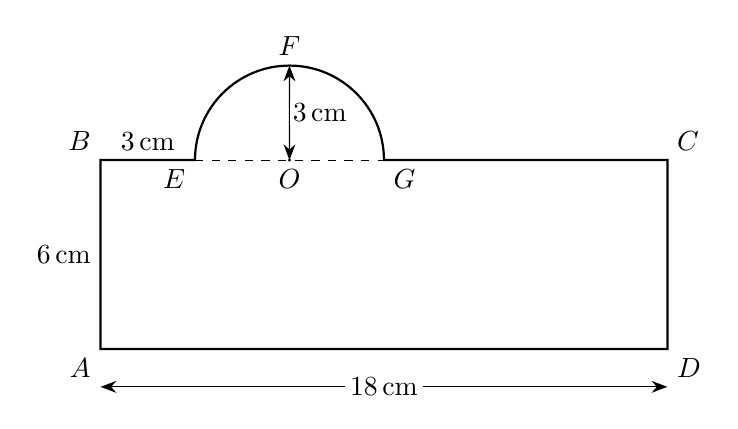
\begin{tikzpicture}[scale=0.4]
\def\W{18}\def\H{6}\def\ox{6}\def\rad{3}\def\dimdrop{1.2}
\coordinate (A) at (0,0);
\coordinate (B) at (0,\H);
\coordinate (C) at (\W,\H);
\coordinate (D) at (\W,0);
\coordinate (O) at (\ox,\H);
\coordinate (E) at ($(O)+(-\rad,0)$);
\coordinate (F) at ($(O)+(0,\rad)$);
\coordinate (G) at ($(O)+(\rad,0)$);
\draw[thick,black] (A)--(B)--(E) arc[start angle=180,end angle=0,radius=\rad] --(C)--(D)--cycle;
\draw[dashed] (E)--(G);
\foreach \p/\pos in {A/below left,B/above left,C/above right,D/below right,E/below left,F/above,G/below right} {\node[\pos] at (\p) {$\p$};}
\fill (O) circle (1.5pt);
\node[below] at (O) {$O$};
\path (A)--(B) node[midway,left] {$6\,\mathrm{cm}$};
\draw[{Stealth[length=2mm]}-{Stealth[length=2mm]}] ($(A)+(0,-\dimdrop)$)--($(D)+(0,-\dimdrop)$) node[midway,fill=white,inner sep=2pt] {$18\,\mathrm{cm}$};
\path (B)--(E) node[midway,above] {$3\,\mathrm{cm}$};
\draw[{Stealth[length=2mm]}-{Stealth[length=2mm]}] (O)--(F) node[midway,right,fill=white,inner sep=1pt] {$3\,\mathrm{cm}$};
\end{tikzpicture}
\end{figure}


\begin{enumerate}[label=\textbf{(\alph*)}]
\item Consider the semicircular tab $EFG$ on its own. Using the standard centre-of-mass result for a uniform semicircular lamina, show that its centre of mass is $1.27\,\mathrm{cm}$ from the diameter $EG$, correct to $3$ significant figures. State the exact distance. \marks{2}

\item For the complete lamina, find
\begin{enumerate}[label=(\roman*)]
\item the distance from $AB$ to its centre of mass, giving your answer exactly, \marks{4}
\item the distance from $AD$ to its centre of mass, giving your answer exactly. \marks{3}
\end{enumerate}

\item The complete lamina has weight $24\,\mathrm{N}$ and is smoothly pivoted at $A$.
A wire attached at $C$ supports it in equilibrium.
The wire pulls upwards and to the left at $30^\circ$ above the horizontal, and its tension is $10\,\mathrm{N}$.

The side $AD$ makes an angle $\theta$ above the horizontal, where $0^\circ<\theta<45^\circ$, as shown in the diagram below.

\begin{figure}[H]
    \centering
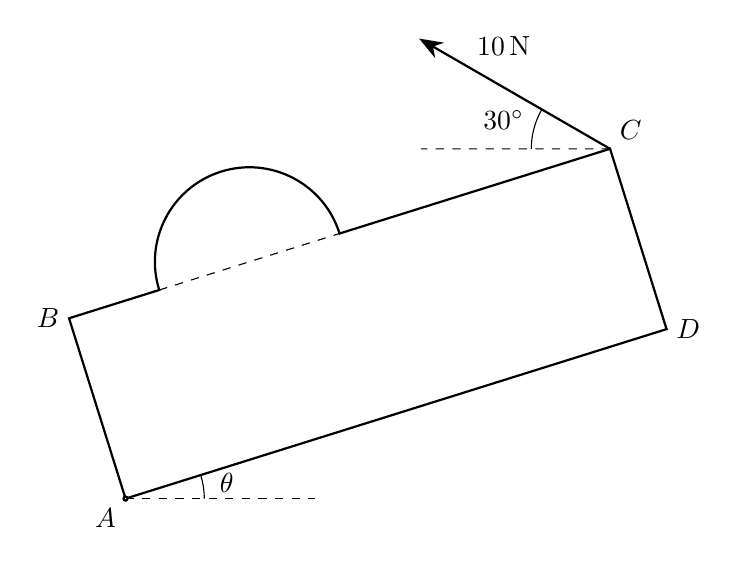
\begin{tikzpicture}[scale=0.4]
\def\W{18}\def\H{6}\def\ox{6}\def\rad{3}\def\wirelen{7}\def\reflen{6}\def\wireang{150}
\pgfmathsetmacro{\area}{\W*\H+pi*\rad^2/2}
\pgfmathsetmacro{\xbar}{(\W*\H*\W/2+(pi*\rad^2/2)*\ox)/\area}
\pgfmathsetmacro{\ybar}{(\W*\H*\H/2+(pi*\rad^2/2)*(\H+4*\rad/(3*pi)))/\area}
\pgfmathsetmacro{\ang}{atan((24*\xbar-10*(\W/2+sqrt(3)*\H/2))/(10*(sqrt(3)*\W/2-\H/2)+24*\ybar))}
\coordinate (A) at (0,0);
\coordinate (X) at (\reflen,0);
\begin{scope}[rotate=\ang]
\coordinate (B) at (0,\H);
\coordinate (C) at (\W,\H);
\coordinate (D) at (\W,0);
\coordinate (O) at (\ox,\H);
\coordinate (E) at ($(O)+(-\rad,0)$);
\coordinate (G) at ($(O)+(\rad,0)$);
\draw[thick,black] (A)--(B)--(E) arc[start angle=180,end angle=0,radius=\rad] --(C)--(D)--cycle;
\draw[dashed] (E)--(G);
\end{scope}
\coordinate (L) at ($(C)+(-\reflen,0)$);
\coordinate (S) at ($(C)+(\wireang:\wirelen)$);
\draw[dashed] (A)--(X);
\draw[dashed] (C)--(L);
\draw[-{Stealth[length=3mm]},thick,black] (C)--(S) node[pos=0.75,above right] {$10\,\mathrm{N}$};
\pic["$\theta$",draw,angle radius=10mm,angle eccentricity=1.3] {angle=X--A--D};
\pic["$30^\circ$",draw,angle radius=10mm,angle eccentricity=1.4] {angle=S--C--L};
\draw[thick,fill=white] (A) circle (1.8pt);
\node[below left] at (A) {$A$};
\node[left] at (B) {$B$};
\node[above right] at (C) {$C$};
\node[right] at (D) {$D$};
\end{tikzpicture}
\end{figure}


Calculate $\theta$, giving your answer to $3$ significant figures. \marks{6}
\end{enumerate}

\vspace*{10pt}

\begin{djsSolution}
\begin{enumerate}[label=\textbf{(\alph*)}, start=1]
\item Consider only the semicircular tab \(EFG\). The centre of mass of a uniform semicircular lamina of radius \(r\) lies on its axis of symmetry, a distance \(\frac{4r}{3\pi}\) from its diameter. Here \(r=3\,\mathrm{cm}\), so the distance from \(EG\) is
\[
\dfrac{4\times3}{3\pi}=\dfrac{4}{\pi}\,\mathrm{cm}\approx1.27\,\mathrm{cm}\qquad\text{(3 s.f.)}
\]

\item
The lamina is uniform, so areas can be used as weights. Let the centre of mass of the complete lamina be at distances \(\bar{x}\) from \(AB\) and \(\bar{y}\) from \(AD\). If piece \(i\) has area \(\mathcal{A}_i\) and its centre of mass is at distances \(x_i\) from \(AB\) and \(y_i\) from \(AD\), then
\[
\mathcal{A}\bar{x}=\sum\mathcal{A}_ix_i,\qquad \mathcal{A}\bar{y}=\sum\mathcal{A}_iy_i
\]

where \(\mathcal{A}=\sum\mathcal{A}_i\).

\begin{enumerate}[label=(\roman*), start=1]
\item The component areas and centre-of-mass distances are
\[
\renewcommand{\arraystretch}{1.5}
\setlength{\arraycolsep}{8pt}
\begin{array}{c|c|c}
\text{Component}&\text{Area }(\mathrm{cm^2})&\text{Distance from }AB\ (\mathrm{cm})\\
\hline
\text{Rectangle}&18\times6=108&\tfrac{18}{2}=9\\
\text{Semicircle}&\tfrac12\pi(3)^2=\tfrac{9\pi}{2}&BE+EO=3+3=6
\end{array}
\]

Taking moments about \(AB\):
\begin{align*}
\left(108+\dfrac{9\pi}{2}\right)\bar{x}
&=108\times9+\dfrac{9\pi}{2}\times6\\
\bar{x}&=\dfrac{972+27\pi}{108+\frac{9\pi}{2}}\\
&=\dfrac{216+6\pi}{24+\pi}\,\mathrm{cm}
\end{align*}

\item The rectangle's centre of mass is \(3\,\mathrm{cm}\) from \(AD\). Using part (a), the semicircle's centre of mass is at distance
\[
\left(6+\dfrac{4}{\pi}\right)\,\mathrm{cm}
\]

Taking moments about \(AD\):
\begin{align*}
\left(108+\dfrac{9\pi}{2}\right)\bar{y}
&=108\times3+\dfrac{9\pi}{2}\left(6+\dfrac{4}{\pi}\right)\\
&=324+27\pi+18\\
\bar{y}&=\dfrac{342+27\pi}{108+\frac{9\pi}{2}}\\
&=\dfrac{76+6\pi}{24+\pi}\,\mathrm{cm}
\end{align*}

\end{enumerate}
\item
Resolve the tension parallel and perpendicular to \(AD\). The angle between the wire and the direction \(DA\) is \(\theta+30^\circ\), so the components are
\begin{align*}
T_{\parallel}&=10\cos(\theta+30^\circ)\,\mathrm{N}
&&\text{in the direction }DA\\
T_{\perp}&=10\sin(\theta+30^\circ)\,\mathrm{N}
&&\text{in the direction }AB
\end{align*}

These components both produce anticlockwise moments about \(A\), with perpendicular distances \(6\,\mathrm{cm}\) and \(18\,\mathrm{cm}\), respectively. The reaction at the pivot has zero moment about \(A\).

After rotation through \(\theta\), the horizontal distance of the centre of mass from \(A\) is \(\bar{x}\cos\theta-\bar{y}\sin\theta\). Taking moments about \(A\), in \(\mathrm{N\,cm}\):
\begin{align*}
10\left[18\sin(\theta+30^\circ)+6\cos(\theta+30^\circ)\right]
&=24(\bar{x}\cos\theta-\bar{y}\sin\theta)\\
18\sin(\theta+30^\circ)+6\cos(\theta+30^\circ)
&=\dfrac{12}{5}(\bar{x}\cos\theta-\bar{y}\sin\theta)
\end{align*}

Expanding the compound angles and collecting terms:
\begin{align*}
18\left(\dfrac{\sqrt3}{2}\sin\theta+\dfrac12\cos\theta\right)
+6\left(\dfrac{\sqrt3}{2}\cos\theta-\dfrac12\sin\theta\right)
&=\dfrac{12}{5}(\bar{x}\cos\theta-\bar{y}\sin\theta)\\
\left(9\sqrt3-3+\dfrac{12\bar{y}}{5}\right)\sin\theta
&=\left(\dfrac{12\bar{x}}{5}-9-3\sqrt3\right)\cos\theta\\
\tan\theta&=\dfrac{\frac{12\bar{x}}{5}-9-3\sqrt3}{9\sqrt3-3+\frac{12\bar{y}}{5}}
\end{align*}

Using the exact values from parts (b)(i) and (b)(ii), and \(0^\circ<\theta<45^\circ\), gives
\[
\theta\approx17.4^\circ\qquad\text{(3 s.f.)}
\]

\end{enumerate}
\end{djsSolution}

\end{enumerate}
\end{document}
